
RPN(逆波兰表达式)计算器是一种基于堆栈的计算器,它使用后缀符号,其中操作符紧跟在操作数之后。它通常用于打印计算器,特别是HP 12C,有史以来最受欢迎的电子计算器。

熟悉了其操作模式后,许多人更喜欢RPN计算器(自从惠普12C和16C在上世纪80年代初首次推出以来,我一直在使用它们)。例如,使用传统的代数符号,要将1和2相加,可以输入1 + 2。使用RPN,可以输入1 2 +。操作符跟在操作数后面。

使用代数计算器,需要按下=键来表示需要一个结果。对于RPN计算器,这是不必要的,因为操作人员立即进行处理,具有双重目的。另一方面,RPN计算器通常需要按回车键将操作数推入堆栈。

我们可以使用基于堆栈的数据结构轻松实现RPN计算器。例如,实现一个具有四个位置堆栈的RPN计算器:

\hspace*{\fill} \\ %插入空行
\begin{center}
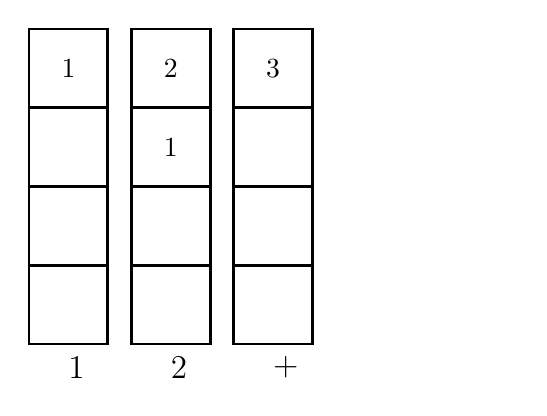
\begin{tikzpicture}
\draw[line width=1pt] (1,-1*0) rectangle (0, -1*0+1) node[pos=.5] {1};
\draw[line width=1pt] (1,-1*1) rectangle (0, -1*1+1);
\draw[line width=1pt] (1,-1*2) rectangle (0, -1*2+1);
\draw[line width=1pt] (1,-1*3) rectangle (0, -1*3+1);

\draw[line width=1pt] (2.3,-1*0) rectangle (1.3, -1*0+1) node[pos=.5] {2};
\draw[line width=1pt] (2.3,-1*1) rectangle (1.3, -1*1+1) node[pos=.5] {1};
\draw[line width=1pt] (2.3,-1*2) rectangle (1.3, -1*2+1);
\draw[line width=1pt] (2.3,-1*3) rectangle (1.3, -1*3+1);

\draw[line width=1pt] (3.6,-1*0) rectangle (2.6, -1*0+1) node[pos=.5] {3};
\draw[line width=1pt] (3.6,-1*1) rectangle (2.6, -1*1+1);
\draw[line width=1pt] (3.6,-1*2) rectangle (2.6, -1*2+1);
\draw[line width=1pt] (3.6,-1*3) rectangle (2.6, -1*3+1);

\node[text width=3cm, font=\large] at (2,-3.3) {1};
\node[text width=3cm, font=\large] at (3.3,-3.3) {2};
\node[text width=3cm, font=\large] at (4.6,-3.3) {+};
\end{tikzpicture}
	
图3.5  RPN的加法操作
\end{center}

每个操作数在输入时压入堆栈。当输入操作符时,操作数弹出,操作,结果压回堆栈。然后,该结果可用于下一个操作。例如,考虑(3+2)×3的情况:

\hspace*{\fill} \\ %插入空行
\begin{center}
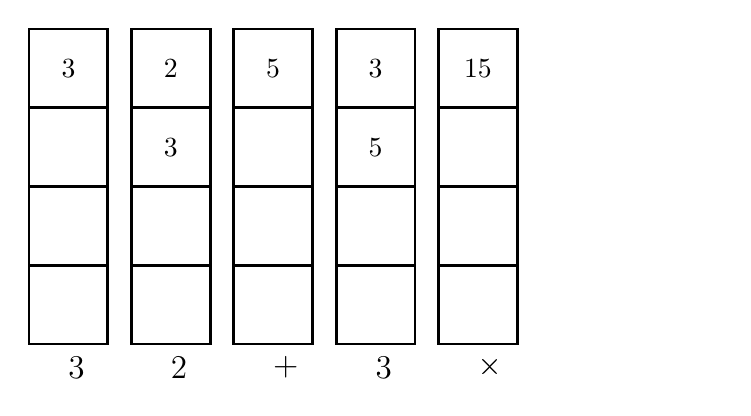
\begin{tikzpicture}
\draw[line width=1pt] (1,-1*0) rectangle (0, -1*0+1) node[pos=.5] {3};
\draw[line width=1pt] (1,-1*1) rectangle (0, -1*1+1);
\draw[line width=1pt] (1,-1*2) rectangle (0, -1*2+1);
\draw[line width=1pt] (1,-1*3) rectangle (0, -1*3+1);

\draw[line width=1pt] (2.3,-1*0) rectangle (1.3, -1*0+1) node[pos=.5] {2};
\draw[line width=1pt] (2.3,-1*1) rectangle (1.3, -1*1+1) node[pos=.5] {3};
\draw[line width=1pt] (2.3,-1*2) rectangle (1.3, -1*2+1);
\draw[line width=1pt] (2.3,-1*3) rectangle (1.3, -1*3+1);

\draw[line width=1pt] (3.6,-1*0) rectangle (2.6, -1*0+1) node[pos=.5] {5};
\draw[line width=1pt] (3.6,-1*1) rectangle (2.6, -1*1+1);
\draw[line width=1pt] (3.6,-1*2) rectangle (2.6, -1*2+1);
\draw[line width=1pt] (3.6,-1*3) rectangle (2.6, -1*3+1);

\draw[line width=1pt] (4.9,-1*0) rectangle (3.9, -1*0+1) node[pos=.5] {3};
\draw[line width=1pt] (4.9,-1*1) rectangle (3.9, -1*1+1) node[pos=.5] {5};
\draw[line width=1pt] (4.9,-1*2) rectangle (3.9, -1*2+1);
\draw[line width=1pt] (4.9,-1*3) rectangle (3.9, -1*3+1);

\draw[line width=1pt] (6.2,-1*0) rectangle (5.2, -1*0+1) node[pos=.5] {15};
\draw[line width=1pt] (6.2,-1*1) rectangle (5.2, -1*1+1);
\draw[line width=1pt] (6.2,-1*2) rectangle (5.2, -1*2+1);
\draw[line width=1pt] (6.2,-1*3) rectangle (5.2, -1*3+1);

\node[text width=3cm, font=\large] at (2,-3.3) {3};
\node[text width=3cm, font=\large] at (3.3,-3.3) {2};
\node[text width=3cm, font=\large] at (4.6,-3.3) {+};
\node[text width=3cm, font=\large] at (5.9,-3.3) {3};
\node[text width=3cm, font=\large] at (7.2,-3.3) {×};
\end{tikzpicture}

图3.6  RPN的堆栈操作
\end{center}

RPN的优点是可以将操作数留在堆栈上以供将来计算,从而减少了对单独内存寄存器的需求。考虑(9×6)+(2×3)的情况:

\hspace*{\fill} \\ %插入空行
\begin{center}
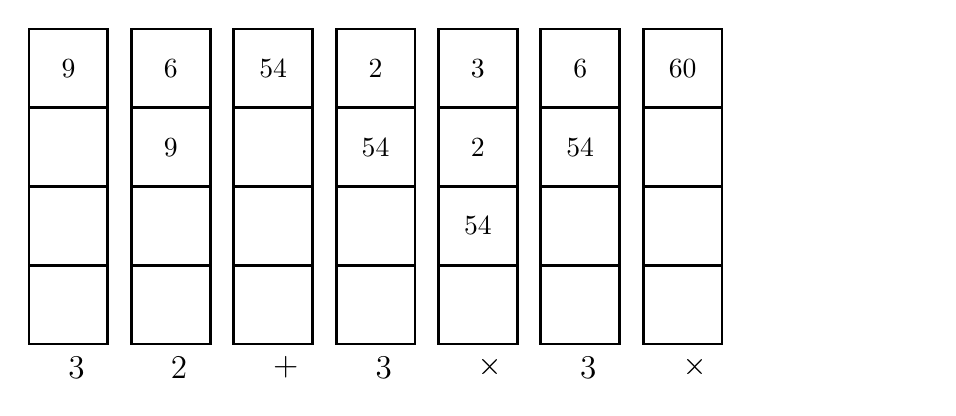
\begin{tikzpicture}
\draw[line width=1pt] (1,-1*0) rectangle (0, -1*0+1) node[pos=.5] {9};
\draw[line width=1pt] (1,-1*1) rectangle (0, -1*1+1);
\draw[line width=1pt] (1,-1*2) rectangle (0, -1*2+1);
\draw[line width=1pt] (1,-1*3) rectangle (0, -1*3+1);

\draw[line width=1pt] (2.3,-1*0) rectangle (1.3, -1*0+1) node[pos=.5] {6};
\draw[line width=1pt] (2.3,-1*1) rectangle (1.3, -1*1+1) node[pos=.5] {9};
\draw[line width=1pt] (2.3,-1*2) rectangle (1.3, -1*2+1);
\draw[line width=1pt] (2.3,-1*3) rectangle (1.3, -1*3+1);

\draw[line width=1pt] (3.6,-1*0) rectangle (2.6, -1*0+1) node[pos=.5] {54};
\draw[line width=1pt] (3.6,-1*1) rectangle (2.6, -1*1+1);
\draw[line width=1pt] (3.6,-1*2) rectangle (2.6, -1*2+1);
\draw[line width=1pt] (3.6,-1*3) rectangle (2.6, -1*3+1);

\draw[line width=1pt] (4.9,-1*0) rectangle (3.9, -1*0+1) node[pos=.5] {2};
\draw[line width=1pt] (4.9,-1*1) rectangle (3.9, -1*1+1) node[pos=.5] {54};
\draw[line width=1pt] (4.9,-1*2) rectangle (3.9, -1*2+1);
\draw[line width=1pt] (4.9,-1*3) rectangle (3.9, -1*3+1);

\draw[line width=1pt] (6.2,-1*0) rectangle (5.2, -1*0+1) node[pos=.5] {3};
\draw[line width=1pt] (6.2,-1*1) rectangle (5.2, -1*1+1) node[pos=.5] {2};
\draw[line width=1pt] (6.2,-1*2) rectangle (5.2, -1*2+1) node[pos=.5] {54};
\draw[line width=1pt] (6.2,-1*3) rectangle (5.2, -1*3+1);

\draw[line width=1pt] (7.5,-1*0) rectangle (6.5, -1*0+1) node[pos=.5] {6};
\draw[line width=1pt] (7.5,-1*1) rectangle (6.5, -1*1+1) node[pos=.5] {54};
\draw[line width=1pt] (7.5,-1*2) rectangle (6.5, -1*2+1);
\draw[line width=1pt] (7.5,-1*3) rectangle (6.5, -1*3+1);

\draw[line width=1pt] (8.8,-1*0) rectangle (7.8, -1*0+1) node[pos=.5] {60};
\draw[line width=1pt] (8.8,-1*1) rectangle (7.8, -1*1+1);
\draw[line width=1pt] (8.8,-1*2) rectangle (7.8, -1*2+1);
\draw[line width=1pt] (8.8,-1*3) rectangle (7.8, -1*3+1);

\node[text width=3cm, font=\large] at (2,-3.3) {3};
\node[text width=3cm, font=\large] at (3.3,-3.3) {2};
\node[text width=3cm, font=\large] at (4.6,-3.3) {+};
\node[text width=3cm, font=\large] at (5.9,-3.3) {3};
\node[text width=3cm, font=\large] at (7.2,-3.3) {×};
\node[text width=3cm, font=\large] at (8.5,-3.3) {3};
\node[text width=3cm, font=\large] at (9.8,-3.3) {×};
\end{tikzpicture}

图3.7  RPN的多栈操作
\end{center}

注意,首先执行括号内的操作,然后对中间结果执行最后的操作。这可能一开始看起来比较复杂,但当习惯了,就很有意义了。

现在,使用STL deque容器构建一个简单的RPN计算器。

\subsubsection{How to do it…}

对于这个实现,我们将为堆栈使用deque容器。为什么不使用stack容器呢?stack类是一个容器适配器,它使用另一个容器(通常是deque)进行存储。就我们的目标而言,stack与deque相比并没有任何明显的优势。deque允许我们遍历和显示RPN堆栈,就像纸带计算器一样。

\begin{itemize}
\item 
我们将把RPN计算器封装在一个类中,这样做有几个优点。封装提供了安全性、可重用性、可扩展性和干净的接口。我们将类命名为RPN:

\begin{lstlisting}[style=styleCXX]
class RPN {
	deque<double> deq_{};
	constexpr static double zero_{0.0};
	constexpr static double inf_
		{ std::numeric_limits<double>::infinity() };
... // public and private members go here
};
\end{lstlisting}

deque数据存储名为deq\_,位于类的private区域。这是我们存储RPN堆栈的地方。

zero\_常量在整个类中都有使用,既作为返回值,也作为比较操作数。常量inf\_用于除零错误。这些常量会声明为constexpr static,因此不会在每个实例中占用空间。

命名私有数据成员时,我喜欢在后面加下划线,以提醒我它们是私有的。

\item 
我们不需要显式构造函数或析构函数,因为deque类管理自己的资源。所以,公共接口只包含三个功能:

\begin{lstlisting}[style=styleCXX]
public:
	// process an operand/operator
	double op(const string & s) {
		if(is_numeric(s)) {
			double v{stod(s, nullptr)};
			deq_.push_front(v);
			return v;
		}
		else return optor(s);
	}
	// empty the stack
	void clear() {
		deq_.clear();
	}
	// print the stack
	string get_stack_string() const {
		string s{};
		for(auto v : deq_) {
			s += format("{} ", v);
		}
		return s;
	}
\end{lstlisting}

double op()函数是RPN类的主要入口点,接受一个字符串,包含数字或操作符。若是数字,则转换为双精度数并压入堆栈。若是一个操作符,则调用optor()来执行该操作。这是这个类的主要逻辑。

void clear()函数只是在deque上调用clear()来清空堆栈。

最后,string get\_stack\_string()函数以字符串形式返回堆栈的内容。

\item 
在private部分中,有为公共接口工作进行支持的工具函数。pop\_get2()函数从堆栈中弹出两个操作数,并将它们作为一对返回,这里使用this作为操作符的操作数:

\begin{lstlisting}[style=styleCXX]
pair<double, double> pop_get2() {
	if(deq_.size() < 2) return {zero_, zero_};
	double v1{deq_.front()};
	deq_.pop_front();
	double v2{deq_.front()};
	deq_.pop_front();
	return {v2, v1};
}
\end{lstlisting}

\item 
is\_numeric()函数的作用是:检查字符串是否完全是数字,也接受小数点字符。

\begin{lstlisting}[style=styleCXX]
bool is_numeric(const string& s) {
	for(const char c : s) {
		if(c != '.' && !std::isdigit(c)) return
		false;
	}
	return true;
}
\end{lstlisting}

\item 
optor()函数执行操作符,使用map容器将操作符映射到相应的lambda函数。

\begin{lstlisting}[style=styleCXX]
double optor(const string& op) {
	map<string, double (*)(double, double)> opmap {
		{"+", [](double l, double r){ return l + r; }},
		{"-", [](double l, double r){ return l - r; }},
		{"*", [](double l, double r){ return l * r; }},
		{"/", [](double l, double r){ return l / r; }},
		{"^", [](double l, double r)
			{ return pow(l, r); }},
		{"%", [](double l, double r)
			{ return fmod(l, r); }}
	};
	if(opmap.find(op) == m.end()) return zero_;
	auto [l, r] = pop_get2();
	// don’t divide by zero
	if(op == "/" && r == zero_) deq_.push_front(inf_);
	else deq_.push_front(opmap.at(op)(l, r));
	return deq_.front();
}
\end{lstlisting}

带有lambda函数的map容器可以快速简便地创建跳转表。

使用map中的find()函数来测试是否有一个有效的操作符。

在对除零进行测试之后,取消对map的引用,并调用操作符。

操作的结果会压入堆栈并返回。

\item 
这些都是RPN类的函数成员,现在可以在main()函数中使用:

\begin{lstlisting}[style=styleCXX]
int main() {
	RPN rpn;
	
	for(string o{}; cin >> o; ) {
		rpn.op(o);
		auto stack_str{rpn.get_stack_string()};
		cout << format("{}: {}\n", o, stack_str);
	}
}
\end{lstlisting}

我们将通过从命令行将字符串输送到程序中来进行测试,使用for循环从cin流中获取每个单词,并将其传递给rpn.op()。我喜欢这里的for循环,因为它很容易包含o变量的作用域。然后在每个命令行项后使用get\_stack\_string()函数打印堆栈。

\item 
可以通过输入这样的表达式来运行程序:

\begin{tcblisting}{commandshell={}}
$ echo "9 6 * 2 3 * +" | ./rpn
9: 9
6: 6 9
*: 54
2: 2 54
3: 3 2 54
*: 6 54
+: 60
\end{tcblisting}
\end{itemize}

这看起来像很多编码,但实际上很简单。加上注释,RPN类的代码不到70行。完整的rpn.cpp源代码在GitHub的库中。

\subsubsection{How it works…}

RPN类首先确定每个输入块的性质。若是一个数字,则压入堆栈。若是操作符,则从堆栈顶部取出两个操作数,进行操作,并将结果推回堆栈。若是不识别的输入,就忽略它。

deque类是一个双端队列。为了将其用作堆栈,我们选择一个端点,并从同一端点进行push和pop。

若确定一个输入是数字,可以将它转换为double,并使用push\_front()将它推到deque的前面。

\begin{lstlisting}[style=styleCXX]
if(is_numeric(s)) {
	double v{stod(s, nullptr)};
	deq_.push_front(v);
	return v;
}
\end{lstlisting}

当需要使用堆栈中的值时,可以将它们从deque的前面弹出。使用front()获取值,然后pop\_front()将其从堆栈中弹出。

\begin{lstlisting}[style=styleCXX]
pair<double, double> pop_get2() {
	if(deq_.size() < 2) return {zero_, zero_};
	double v1{deq_.front()};
	deq_.pop_front();
	double v2{deq_.front()};
	deq_.pop_front();
	return {v2, v1};
}
\end{lstlisting}

为操作符使用map使得检查操作符是否有效和执行操作变得容易。

\begin{lstlisting}[style=styleCXX]
map<string, double (*)(double, double)> opmap {
	{"+", [](double l, double r){ return l + r; }},
	{"-", [](double l, double r){ return l - r; }},
	{"*", [](double l, double r){ return l * r; }},
	{"/", [](double l, double r){ return l / r; }},
	{"^", [](double l, double r){ return pow(l, r); }},
	{"%", [](double l, double r){ return fmod(l, r); }}
};
\end{lstlisting}

可以使用find()函数来测试操作符的有效性:

\begin{lstlisting}[style=styleCXX]
if(opmap.find(op) == opmap.end()) return zero_;
\end{lstlisting}

可以通过使用at()函数对map进行解引用来调用该操作符:

\begin{lstlisting}[style=styleCXX]
opmap.at(op)(l, r)
\end{lstlisting}

这里调用运算符lambda,并在一条语句中将结果推入deque:

\begin{lstlisting}[style=styleCXX]
deq_.push_front(opmap.at(op)(l, r));
\end{lstlisting}

\subsubsection{There's more…}

在这个示例中,我们使用cin流向RPN计算器提供操作。使用STL容器同样可以做到这一点。

\begin{lstlisting}[style=styleCXX]
int main() {
	RPN rpn;
	vector<string> opv{ "9", "6", "*", "2", "3", "*", "+"
	};
	for(auto o : opv) {
		rpn.op(o);
		auto stack_str{rpn.get_stack_string()};
		cout << format("{}: {}\n", o, stack_str);
	}
}
\end{lstlisting}

输出:

\begin{tcblisting}{commandshell={}}
9: 9
6: 6 9
*: 54
2: 2 54
3: 3 2 54
*: 6 54
+: 60
\end{tcblisting}

通过将RPN计算器放在一个清晰接口的类中,我们创建了一个可以在许多不同上下文中使用的灵活工具。







